\documentclass[11pt]{article}

% ============================================================
% Packages
% ============================================================
\usepackage[utf8]{inputenc}
\usepackage[margin=1in]{geometry}
\usepackage{amsmath,amssymb,amsthm}
\usepackage{graphicx}
\usepackage{booktabs}
\usepackage{xcolor}
\usepackage{hyperref}
\usepackage{tikz}
\usepackage{enumitem}
\usepackage{pgfplots}

\pgfplotsset{compat=1.18}

% ============================================================
% Document Formatting
% ============================================================
\setlength{\parskip}{0.6em}
\setlength{\parindent}{0pt}

% ============================================================
% List Formatting
% ============================================================
\setlist[enumerate]{
    leftmargin=2em,
    itemsep=0.25em
}

% ============================================================
% Solution Environment
% ============================================================
\newenvironment{solution}
    {\par\noindent\textbf{Solution.}\par}
    {\par}

% ============================================================
% Link Styling
% ============================================================
\hypersetup{
    colorlinks=true,
    linkcolor=blue,
    urlcolor=cyan
}

% ============================================================
% Metadata
% ============================================================
\title{Ordinary Differential Equations}
\author{Chris Ritter}
\date{August 25, 2026}

% ============================================================
% Document
% ============================================================

\begin{document}

\maketitle
\tableofcontents
\newpage

% ============================================================
\section{Solutions of Differential Equations}
% ============================================================

Consider an \(n\)th-order differential equation of the form
\[
y^{(n)}
=
f\left(t,y,y',\ldots,y^{(n-1)}\right),
\]
where \(y=y(t)\).

\subsection{Definition of a Solution}

A solution of this differential equation on an interval
\[
\alpha < t < \beta
\]
is a function
\[
y=\phi(t)
\]
such that
\[
\phi',\phi'',\ldots,\phi^{(n)}
\]
exist and
\[
\phi^{(n)}(t)
=
f\left(
t,\phi(t),\phi'(t),\ldots,\phi^{(n-1)}(t)
\right)
\]
for every \(t\) in the interval \((\alpha,\beta)\).

In other words, a solution is a function that satisfies the differential equation at every point in the interval under consideration.

\subsection{Example}

Consider the second-order differential equation
\[
y''+y=0.
\]

Equivalently,
\[
y''=-y.
\]

Two solutions are
\[
y_1(t)=\cos t
\]
and
\[
y_2(t)=\sin t.
\]

For \(y_1\),
\[
y_1'(t)=-\sin t,
\qquad
y_1''(t)=-\cos t=-y_1(t).
\]

For \(y_2\),
\[
y_2'(t)=\cos t,
\qquad
y_2''(t)=-\sin t=-y_2(t).
\]

Thus both functions satisfy the differential equation for
\[
-\infty<t<\infty.
\]

Furthermore, because the differential equation is linear, any linear combination of these solutions is also a solution. Thus
\[
y(t)=c_1\cos t+c_2\sin t
\]
is a solution for any constants \(c_1,c_2\in\mathbb{R}\).

Therefore, this differential equation has infinitely many solutions.

The constants \(c_1\) and \(c_2\) allow us to select different solutions from this family.

% ============================================================
\section{First-Order Equations}
% ============================================================

A first-order differential equation has the general form
\[
y'=f(t,y).
\]

Two fundamental questions are:

\begin{enumerate}
    \item Does a solution exist?
    \item If a solution exists, is it unique?
\end{enumerate}

These questions are central to the theory of differential equations.

There are several important types of first-order differential equations. In this course, we will consider:

\begin{enumerate}
    \item linear equations,
    \item separable equations,
    \item exact equations.
\end{enumerate}

% ============================================================
\section{First-Order Linear Equations}
% ============================================================

A first-order linear differential equation can be written in the form
\[
y'+p(t)y=g(t),
\]
where \(p(t)\) and \(g(t)\) are known functions.

Equivalently,
\[
y'=-p(t)y+g(t).
\]

When \(p(t)=a\) and \(g(t)=b\) are constants, we obtain
\[
y'+ay=b.
\]

This is called a first-order linear differential equation with constant coefficients.

For now, assume
\[
a\neq 0.
\]

\subsection{The Integrating Factor}

We want to solve
\[
y'+ay=b.
\]

The main idea is to multiply the entire equation by a carefully chosen function
\[
\mu(t),
\]
called an \textbf{integrating factor}.

Multiplying by \(\mu(t)\) gives
\[
\mu y'+a\mu y=\mu b.
\]

We want the left-hand side to become the derivative of the product
\[
\mu y.
\]

By the product rule,
\[
\frac{d}{dt}(\mu y)
=
\mu' y+\mu y'.
\]

Therefore, we need
\[
\mu' y+\mu y'
=
\mu y'+a\mu y.
\]

Comparing the two expressions, we require
\[
\mu'=a\mu.
\]

Thus \(\mu\) must satisfy the differential equation
\[
\frac{d\mu}{dt}=a\mu.
\]

Separating variables,
\[
\frac{d\mu}{\mu}=a\,dt.
\]

Integrating,
\[
\int\frac{1}{\mu}\,d\mu
=
\int a\,dt,
\]
so
\[
\ln|\mu|=at+C.
\]

Exponentiating,
\[
|\mu|=Ce^{at}.
\]

Since any nonzero constant multiple of an integrating factor is also an integrating factor, we may choose
\[
\boxed{\mu(t)=e^{at}}.
\]

Thus \(e^{at}\) is the integrating factor for
\[
y'+ay=b.
\]

\subsection{Solving the Equation}

Multiply
\[
y'+ay=b
\]
by the integrating factor
\[
e^{at}.
\]

We obtain
\[
e^{at}y'+ae^{at}y
=
be^{at}.
\]

By the product rule,
\[
\frac{d}{dt}\left(e^{at}y\right)
=
be^{at}.
\]

Integrating both sides,
\[
\int
\frac{d}{dt}\left(e^{at}y\right)\,dt
=
\int be^{at}\,dt.
\]

Therefore,
\[
e^{at}y
=
b\int e^{at}\,dt+C.
\]

Since \(a\neq 0\),
\[
\int e^{at}\,dt
=
\frac{1}{a}e^{at}.
\]

Hence
\[
e^{at}y
=
\frac{b}{a}e^{at}+C.
\]

Dividing by \(e^{at}\),
\[
y
=
\frac{b}{a}+Ce^{-at}.
\]

Therefore, the general solution is

\[
\boxed{
y(t)=\frac{b}{a}+Ce^{-at}
}.
\]

\subsection{Initial Conditions}

Suppose we are given the initial condition
\[
y(0)=y_0.
\]

Substituting \(t=0\) into the general solution,
\[
y_0
=
\frac{b}{a}+Ce^0.
\]

Thus
\[
y_0=\frac{b}{a}+C,
\]
so
\[
C=y_0-\frac{b}{a}.
\]

Therefore, the solution to the initial-value problem
\[
y'+ay=b,
\qquad
y(0)=y_0
\]
is

\[
\boxed{
y(t)
=
\frac{b}{a}
+
\left(
y_0-\frac{b}{a}
\right)e^{-at}
}.
\]

Notice that
\[
\frac{b}{a}
\]
is the equilibrium solution. The term
\[
\left(
y_0-\frac{b}{a}
\right)e^{-at}
\]
describes how the solution differs from equilibrium based on the initial condition.

% ============================================================
\section{Example}
% ============================================================

Consider the initial-value problem
\[
\frac{dy}{dt}+2y=3,
\qquad
y(0)=y_0.
\]

Here,
\[
a=2,
\qquad
b=3.
\]

The integrating factor is
\[
\mu(t)=e^{2t}.
\]

Multiplying the differential equation by \(e^{2t}\),
\[
e^{2t}\frac{dy}{dt}
+
2e^{2t}y
=
3e^{2t}.
\]

Using the product rule,
\[
\frac{d}{dt}\left(e^{2t}y\right)
=
3e^{2t}.
\]

Integrating,
\[
e^{2t}y
=
\int 3e^{2t}\,dt
=
\frac{3}{2}e^{2t}+C.
\]

Therefore,
\[
y
=
\frac{3}{2}
+
Ce^{-2t}.
\]

Applying the initial condition \(y(0)=y_0\),
\[
y_0
=
\frac{3}{2}+C.
\]

Thus
\[
C=y_0-\frac{3}{2}.
\]

Hence the solution is

\[
\boxed{
y(t)
=
\frac{3}{2}
+
\left(
y_0-\frac{3}{2}
\right)e^{-2t}
}.
\]

% ============================================================
\section{General First-Order Linear Equation}
% ============================================================

The same method works for the more general first-order linear equation
\[
y'+p(t)y=g(t).
\]

We seek an integrating factor \(\mu(t)\) such that
\[
\mu y'+\mu p(t)y
\]
is the derivative of \(\mu y\).

Since
\[
\frac{d}{dt}(\mu y)
=
\mu'y+\mu y',
\]
we require
\[
\mu'=p(t)\mu.
\]

Separating variables,
\[
\frac{d\mu}{\mu}=p(t)\,dt.
\]

Integrating,
\[
\ln|\mu|
=
\int p(t)\,dt.
\]

Thus we may choose
\[
\boxed{
\mu(t)
=
e^{\int p(t)\,dt}
}.
\]

Multiplying the original equation by \(\mu(t)\),
\[
\mu y'+\mu p(t)y
=
\mu g(t).
\]

The left-hand side becomes
\[
\frac{d}{dt}\left(\mu y\right),
\]
so
\[
\frac{d}{dt}\left(\mu y\right)
=
\mu g(t).
\]

Integrating,
\[
\mu(t)y(t)
=
\int \mu(t)g(t)\,dt+C.
\]

Therefore,

\[
\boxed{
y(t)
=
\frac{
\displaystyle
\int \mu(t)g(t)\,dt+C
}{
\mu(t)
}
}
\]

where
\[
\boxed{
\mu(t)=e^{\int p(t)\,dt}
}.
\]

This is the general integrating-factor method for first-order linear differential equations.

% ============================================================
\section{The Integrating Factor Method}
% ============================================================

Consider the first-order linear differential equation
\[
y'+p(t)y=g(t).
\]

We seek a function
\[
\mu=\mu(t)
\]
called an \textbf{integrating factor} such that, after multiplying the
differential equation by \(\mu(t)\), the left-hand side becomes the
derivative of the product \(\mu(t)y(t)\).

Multiplying the equation by \(\mu(t)\),
\[
\mu y'+\mu p(t)y=\mu g(t).
\]

By the product rule,
\[
\frac{d}{dt}\bigl(\mu y\bigr)
=
\mu' y+\mu y'.
\]

Therefore, we want
\[
\mu' y+\mu y'
=
\mu y'+\mu p(t)y.
\]

This will occur provided that
\[
\mu'=p(t)\mu.
\]

Thus, the integrating factor must satisfy
\[
\frac{d\mu}{dt}=p(t)\mu(t).
\]

Separating variables,
\[
\frac{d\mu}{\mu}=p(t)\,dt.
\]

Integrating,
\[
\int\frac{d\mu}{\mu}
=
\int p(t)\,dt,
\]
so
\[
\ln|\mu|
=
\int p(t)\,dt+C.
\]

Exponentiating,
\[
|\mu|
=
e^C e^{\int p(t)\,dt}.
\]

Since a nonzero constant multiple of an integrating factor is also an
integrating factor, we may choose
\[
\boxed{
\mu(t)=e^{\int p(t)\,dt}
}.
\]

\subsection{Solving the Differential Equation}

Multiplying
\[
y'+p(t)y=g(t)
\]
by the integrating factor gives
\[
\mu y'+\mu p(t)y=\mu g(t).
\]

By construction,
\[
\frac{d}{dt}\bigl(\mu y\bigr)=\mu g(t).
\]

Integrating,
\[
\mu(t)y(t)
=
\int \mu(t)g(t)\,dt+C.
\]

Therefore,
\[
\boxed{
y(t)
=
\frac{
\displaystyle
\int \mu(t)g(t)\,dt+C
}{
\mu(t)
}
}.
\]

This gives the general solution of the first-order linear differential
equation.

\subsection{Initial-Value Problems}

Suppose we are given the initial condition
\[
y(t_0)=y_0.
\]

It is often convenient to write the solution using a definite integral.
Choose the integrating factor so that
\[
\mu(t)
=
e^{\int_{t_0}^{t}p(s)\,ds}.
\]

Then
\[
\mu(t_0)=1.
\]

Since
\[
\frac{d}{dt}\bigl(\mu(t)y(t)\bigr)
=
\mu(t)g(t),
\]
integrating from \(t_0\) to \(t\) gives
\[
\mu(t)y(t)-\mu(t_0)y(t_0)
=
\int_{t_0}^{t}\mu(s)g(s)\,ds.
\]

Using
\[
\mu(t_0)=1
\qquad\text{and}\qquad
y(t_0)=y_0,
\]
we obtain
\[
\mu(t)y(t)
=
y_0+\int_{t_0}^{t}\mu(s)g(s)\,ds.
\]

Therefore, the solution to the initial-value problem is

\[
\boxed{
y(t)
=
\frac{
\displaystyle
y_0+
\int_{t_0}^{t}\mu(s)g(s)\,ds
}{
\mu(t)
}
},
\]
where
\[
\boxed{
\mu(t)
=
e^{\int_{t_0}^{t}p(s)\,ds}
}.
\]

% ============================================================
\subsection{Example 1: A Simple Integrating Factor}
% ============================================================

Consider the differential equation
\[
t^2\frac{dy}{dt}+2ty=0.
\]

For \(t\neq 0\), divide by \(t^2\):
\[
\frac{dy}{dt}+\frac{2}{t}y=0.
\]

Here,
\[
p(t)=\frac{2}{t}.
\]

The integrating factor is
\[
\mu(t)
=
e^{\int \frac{2}{t}\,dt}
=
e^{2\ln|t|}
=
t^2.
\]

Thus,
\[
t^2\frac{dy}{dt}+2ty=0
\]
can be written as
\[
\frac{d}{dt}\left(t^2y\right)=0.
\]

Integrating,
\[
t^2y=C.
\]

Therefore,
\[
\boxed{
y(t)=\frac{C}{t^2}
},
\qquad t\neq 0.
\]

The solution is defined separately on intervals that do not contain
\(t=0\), such as
\[
(-\infty,0)
\qquad\text{or}\qquad
(0,\infty).
\]

% ============================================================
\subsection{Example 2: Solving an Initial-Value Problem}
% ============================================================

Consider the initial-value problem
\[
t\frac{dy}{dt}+2y=4t^2,
\qquad
y(1)=2.
\]

First divide by \(t\), assuming \(t\neq 0\):
\[
\frac{dy}{dt}+\frac{2}{t}y=4t.
\]

Thus,
\[
p(t)=\frac{2}{t},
\qquad
g(t)=4t.
\]

The integrating factor is
\[
\mu(t)
=
e^{\int \frac{2}{t}\,dt}.
\]

Since the initial condition is given at \(t=1\), we are working on the
interval \(t>0\). Therefore,
\[
\mu(t)
=
e^{2\ln t}
=
t^2.
\]

Multiplying the differential equation by \(t^2\),
\[
t^2\frac{dy}{dt}+2ty
=
4t^3.
\]

The left-hand side is the derivative of \(t^2y\):
\[
\frac{d}{dt}\left(t^2y\right)
=
4t^3.
\]

Integrating,
\[
t^2y
=
\int 4t^3\,dt
=
t^4+C.
\]

Therefore,
\[
y
=
t^2+\frac{C}{t^2}.
\]

Apply the initial condition
\[
y(1)=2.
\]

Then
\[
2
=
1+\frac{C}{1^2},
\]
so
\[
C=1.
\]

Hence the unique solution to the initial-value problem is

\[
\boxed{
y(t)=t^2+\frac{1}{t^2}
},
\qquad t>0.
\]

\subsection{Behavior of the Solution}

The solution
\[
y(t)=t^2+\frac{1}{t^2}
\]
has the following limiting behavior.

As \(t\to\infty\),
\[
\lim_{t\to\infty}y(t)
=
\infty,
\]
and more specifically,
\[
\lim_{t\to\infty}\frac{y(t)}{t^2}=1.
\]

Thus, for large positive \(t\),
\[
y(t)\sim t^2.
\]

As \(t\to0^+\),
\[
\lim_{t\to0^+}y(t)
=
\infty,
\]
because
\[
\frac{1}{t^2}\to\infty.
\]

For example, at
\[
t=0.0001,
\]
we have
\[
y(0.0001)
=
(0.0001)^2+\frac{1}{(0.0001)^2}
=
10^{-8}+10^8
\approx 100000000.
\]

Thus, the solution grows extremely rapidly as \(t\) approaches \(0\) from
the right.

% ============================================================
\subsection{Integral Curves}
% ============================================================

The family of solutions
\[
y(t)=t^2+\frac{C}{t^2}
\]
consists of integral curves of the differential equation
\[
t\frac{dy}{dt}+2y=4t^2.
\]

For the initial condition \(y(1)=2\), we obtain the particular solution
\[
y(t)=t^2+\frac{1}{t^2}.
\]

The graph below shows several integral curves corresponding to different
values of \(C\).

\begin{center}
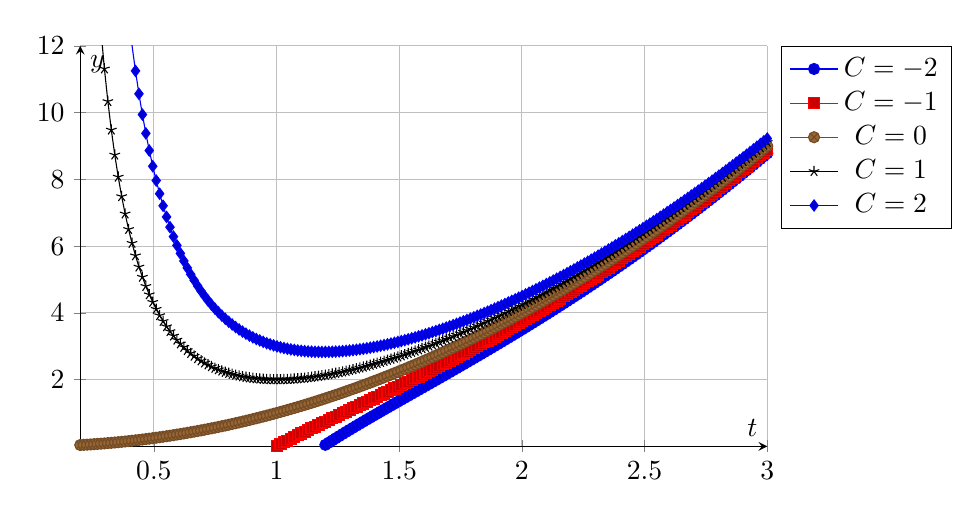
\begin{tikzpicture}
    \begin{axis}[
        width=0.85\textwidth,
        height=0.55\textwidth,
        axis lines=middle,
        xlabel={$t$},
        ylabel={$y$},
        xmin=0.2,
        xmax=3,
        ymin=0,
        ymax=12,
        samples=200,
        domain=0.2:3,
        legend style={
            at={(1.02,1)},
            anchor=north west
        },
        grid=major
    ]

    \addplot {x^2 - 2/x^2};
    \addlegendentry{$C=-2$}

    \addplot {x^2 - 1/x^2};
    \addlegendentry{$C=-1$}

    \addplot {x^2};
    \addlegendentry{$C=0$}

    \addplot {x^2 + 1/x^2};
    \addlegendentry{$C=1$}

    \addplot {x^2 + 2/x^2};
    \addlegendentry{$C=2$}

    \end{axis}
\end{tikzpicture}
\end{center}

The solution corresponding to the initial condition \(y(1)=2\) is the
curve with
\[
C=1.
\]

\end{document}
